\documentclass[a4paper,14pt]{extarticle}
%\makeatletter
%\makeatother
\usepackage[margin=1in]{geometry}
\usepackage{subcaption}
\usepackage{multirow}
\usepackage{graphicx}
%%
%%\usepackage{color}
%%\usepackage{minted}
%%\usepackage[russian]{hyperref}
%%
\graphicspath{{./pictures/}}
\DeclareGraphicsExtensions{.pdf,.png,.jpg}

\usepackage[T2A]{fontenc} 
\usepackage[utf8]{inputenc} % указать кодировку русского текста
\usepackage[english, russian]{babel} % указать, что язык текста - русский
\usepackage{amsmath, amsfonts, amssymb, amsthm,mathtools}
\usepackage[shortcuts,cyremdash]{extdash}
%\usepackage{fancyhdr}
%\pagestyle{fancy}
\begin{document}



\begin{titlepage}
\begin{center}

\textsc{\LARGE Московский\\[-0.2cm]Физико-Технический Институт\\[0.1cm]\large (национальный исследовательский университет)}\\[1.5cm] 


\includegraphics[width=0.3\textwidth]{logo}

\textsc{\Large Лабораторная работа 5.4.1: \\ }

% Title
\HRule \\[0.4cm]
{ \LARGE \bfseries Определение энергии $\alpha$ - частиц по величине их пробега в воздухе. }

\HRule \\[1.5cm]

% Author and supervisor
\noindent
\begin{minipage}{0.4\textwidth}
\begin{flushleft} \large
\end{flushleft}
\end{minipage}%
\begin{minipage}{0.4\textwidth}
\begin{flushright} \large
\end{flushright}
\end{minipage}

\large{\begin{flushright}
\vfill
\textbf{Выполнил}:\\
\textbf{Маслюк Руслан\\}
\textbf{группа Б05-871}
\end{flushright}}

{\large \today}\\

\end{center}
\end{titlepage}











\section{Цель} % (fold)
\label{sec:цель}
Измерить пробег $\alpha$-частиц в воздухе двумя способами:
\begin{itemize}
	\item с помощью сцинтилляционного счетчика
	\item с помощью ионизационной камеры
\end{itemize}
и по полученным величинам определить их энергию.
% section цель (end)

\section{Теоритическая часть} % (fold)
\label{sec:Теоритическая_часть}
	При $\alpha$-распаде исходное материнское ядро испускает ядро гелия ($\alpha$-частицу) и превращается в дочернее ядро, число протонов и число нейтронов которого уменьшается на две единицы. Диапазон изменения энергии вылетающих $\alpha$-частиц значительно меньше - от 4 до 9 МэВ, причем чем меньше их энергия тем больше период полураспада. Функциональная связь между энергией $E$ $\alpha$-частицы и периодом полураспада радиоактивного ядра $T_{\frac{1}{2}}$ хорошо описывается формулой
$$\lg{T_{\frac{1}{2}}}=\frac{a}{\sqrt{E}}+b$$
полученной на основе экспериментальных данных Х.Гейгером и Дж.Нэттолом в 1911 г.

Согласно формуле: $a \simeq 1,6Z; b \simeq-1,6Z^{\frac{2}{3}}-21,4$, вероятность вылета $\alpha$-частицы из ядра определяется вероятностью ее проникновения сквозь кулоновский барьер. Экспоненциальный характер этого процесса возникает вследствие экспоненциального затухания волновой функции в области под барьером, где потенциальная энергия больше энергии частицы.

Экспериментально энергию $\alpha$-частиц удобно определять по величине их пробега в веществе. Тяжелые заряженные частицы с малым зарядом ($z-1, 2$, т.е. протоны и $\alpha$-частицы) при прохождении в веществе теряют свою энергию главным образом в результате неупругих столкновений с атомами вещества. Эти неупругие столкновения вызывают ионизацию и воздбуждение атомов, и поэтому такие потери называются ионизационными. Этот процесс можно рассматривать практически как непрерывный процесс замедления заряженных частиц, поскольку в каждом соударении теряется малая энергия. Энергия, которую можно передать электрону, не превышает $\frac{4mE}{M}$, где $m$ - масса электрона, $M$ - масса заряженный частицы, $E$ - её кинетическая энергия, поэтому частица в результате одного акта такого взаимодействия отклоняется на очень малый угол, максимальное значение которого равно $\frac{m}{M}$, так что практически вся ее траектория в веществе является прямолинейной.

Ядерные взаимодействия в процессах потери энергии заряженной частицей начинают вносить заметный вклад при достаточно высоких энергиях, когда энергия заряженной частицы выше кулоновского барьера. Энергия вылетающих из радиоактивных ядер $\alpha$-частиц принципиально ниже кулоновского барьера, так что для них вероятность ядерных реакций ничтожна. Таким образом, действительно для нерялитивистских тяжелых заряженных частиц основной причиной потери жнергии являются неупругие кулоновские взаимодействия с атомами вещества.
\subsection{Расчет удельных потерь энергии заряженнй частицы в результате взаимодействия с электронами}

Был впервые проведен Н.Бором. Предположим, что частица с зарядом $z$, движущаяся в направлении $x$, проходит на расстоянии $y$ (прицельный параметр) от покоящегося свободного электрона. Атомные электроны можно считать свободными в силу того, что энергия налетающей частицы, согласно нашим предположениям, значительно превышает энергию связи электронов в атомах. В этих условиях электрону передается только импульс в перпендикулярном к движению частицы направлении, который по порядку величины равен произведению электростатической силы ($\frac{ze^2}{y^2}$) на время ее действия ($\sim \frac{2y}{v}$). Следовательно, приобретенная электроном при столкновении энергия $E_e$ будет определяться выражением 
$$E_e=\frac{p^2}{2m}=\Big(\frac{ze^2}{y^2}\frac{2y}{v}\Big)^2\frac{1}{2m}=\frac{2e^4z^2}{mv^2y^2} $$

Если плотность электронов в среде $n_e=nZ$ ($n$ - плотность атомов среды, $Z$ - их заряд), то потеря энергии заряженной частицей на единице пути в результате ее взаимодействия с электронами в слое $2\pi dy$ равна
$$dE(y)=\frac{4\pi n Zz^2e^4}{mv^2}\frac{dy}{y} $$

Полная потеря энергии на единице пути в результате взаимодействия со всеми электронами, расположенными на любых возможных прицельных расстояниях $y$, определеяется интегрированием выражения $(3)$
$$\Big(\frac{dE}{dx}\Big)_{ион}\simeq 4\pi \frac{e^4z^2}{mv^2}nZ\ln{\frac{y_{max}}{y_{min}}} $$

При интегрировании по всей плоскости, перпендикулярной направлению движения, от 0 до  $\infty$ мы получили бы физически абсурдный результат - частица мгновенно тормозится. Поэтому мы ввели ограниченные пределы.

Предельные значения прицельного параметра в $(4)$, полученного в предположении взаимодействия заряженной частицы со свободными электронами, можно определить из следующих соображений. Заметим, что, как следует из $(2)$, энергия, потерянная заряженной частицей при столкновении со свободным электроном, обратно пропорциональна квадрату прицельного параметра, т.е.
$$2\ln{\frac{y_{max}}{y_{min}}}=-\ln{\frac{E_{max}}{E_{min}}} $$

Из закона сохранения энергии следует, что
$$E_{max}=\frac{4mE}{M}=2mv^2 $$

Действительно, в системе покоя частицы электрон в лучшем случае может отскочить от нее, как от абсолютно упругой стенки, т.е. изменить скорость на $2v$. Минимальная энергия, передаваемая электрону в случае связанных электронов, определеяется энергией возбуждения или энергией связи электрона, которые отличаются для электронов различных оболочек. Для определенного вида атомов или молекул это минимальное значение потерянной энергии характеризуют так называемым средним ионизационным потенциалом $\overline{I}$. Таким образом,
$$\ln{\frac{E_{max}}{E_{min}}}=\ln{\frac{2mv^2}{\overline{I}}} $$

а значит, формула для ионизационных потерь нерелятивистской тяжелой 
заряженной частицы имеет вид
$$-\Big(\frac{dE}{dx}\Big)_{ион} \simeq 2\pi \frac{e^4z^2}{mv^2}nZ\ln{\frac{2mv^2}{\overline{I}}} $$

Величину $\frac{dE}{dx}$ называют тормозной способностью вещества.

Мы видим, что из многих параметров, описывающих свойства и движение ионизирующей частицы, в формулу $(8)$ входит только ее заряд и скорость. При данном заряде потери энергии определяются только скоростью частицы, причем с увеличением скорости потери уменьшаются. Быстрее всего теряют энергию медленные частицы.

\subsection{Кривые Брэгга}

Зависимость $\frac{dE}{dx}$ от пути, пройденного частицей в веществе, носит название кривой Брэгга. Две такие кривые движения в воздухе $\alpha$- на рис.1. Как видно из рисунка, кривые Брэгга имеют в конце пробега характерный подъем, называемый пиком Брэгга.

\begin{figure}[h!]
	\centering
	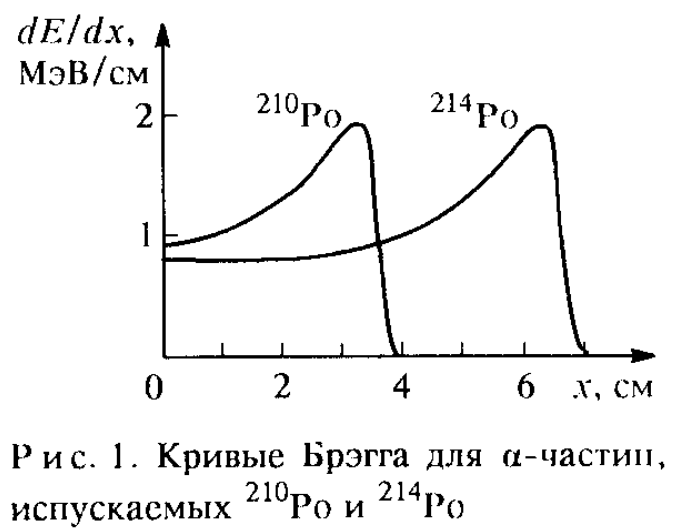
\includegraphics[width = 0.5\linewidth]{Bregg}
\end{figure}

Как отмечалось выше, путь тяжелых заряженных частиц в веществе практически прямолинеен, а разброс длин путей, обусловленный многократным кулоновским рассеянием на ядрах, невелик, и поэтому можно говорить о длине пробега зяраженных частиц в веществе.

Зная зависимость тормозной способности данного вещества от энергии частицы, нетрудно вычислить длину пробега частицы, замедлившейся от начальной энергии $E_0$ до конечной $E_1$. Длину пробега частицы с зарядом $z$ и массой $M$ в веществе с атомным номером $Z$ можно записать в виде:
$$R_{zM}=-\int_{E_1}^{E_0}\frac{dE}{\big(\frac{dE}{dx}\big)}=\frac{m}{2\pi e^4z^2nZ}\int_{E_1}^{E_0}\frac{v^2dE}{\ln{\big(\frac{2mv^2}{\overline{I}}\big)}} $$

Принимая во внимание, что $dE=Mvdv$, получаем
$$R_{zM}=\frac{m}{2\pi e^4z^2nZ}\int_{v_1}^{v_0}\frac{v^3dv}{\ln{\big(\frac{2mv^2}{\overline{I}}\big)}} $$

Существенно, что эта функция для заданной среды одинакова для всех частиц. Если пренебречь слабой логарифмической зависимостью частицы, то
$$R \propto \frac{M}{z^2}v^4_0 \propto E^2 $$

Однако эта формула в силу сделанных предположений недостаточно хорошо описывает экспериментальные данные. Получить хорошее количественное согласие с экспериментальными данными при учете взаимодействия проходящей частицы только с электронами не удается. Поэтому для связи между энергией $\alpha$-частицы и ее пробегом пользуются эмпирическими соотношениями. В диапазоне энергий $\alpha$-частиц от 4 до 9 МэВ эта связь хорошо описывается выражением
$$R=0.32E^{\frac{3}{2}} $$

В этой формуле пробег $\alpha$-частиц в воздухе $R$ (при $15 \; ^\circ C$ и нормальном атмосферном давлении) выражается в сантиметрах, а энергия $E$ - в мегаэлектрон-вольтах. Пробеги $\alpha$-частиц в воздухе для всех радиактивных веществ составляют несколько сантиметров.

Формула $(8)$ показывает, что при данной скорости потери энергии пропорциональны произведению плотности электронов на длину пути: $\Delta E \propto n_e \Delta x$. В заданной среде плотность электронов пропорциональна обычной плотности:
$$n_e=\rho N_A \frac{Z}{A} $$
 
где $N_A$ - постоянная Авогадро, $A$ - атомная масса вещества, $Z$ - атомный номер ээлемента. Поэтому энергия терямая $\alpha$-частицей при прохождении некоторого слоя вещества, определяется произведение $\rho x$, где $\rho$ - плотность вещества, а $x$ - толщина пройденного слоя. Другими словами, энергию частиц удобнее определять не пробегом, выраженным в сантиметрах, а произведением плотности среды на пробег: $R'=\rho R$. Легко видеть, что величина $R'$ имееть размерность $\frac{г}{см^2}$. Она равна массе цилиндра с основанием 1 $см^2$ и длиной, равной пробегу $\alpha$-частиц. Величину $R'$ также принято называть пробегом. Таким образом, пробеги можно выражать в см или $\frac{г}{см^2}$.

Рассеяние  $\alpha$-частиц в веществе и статистический характер потерь энергии приводят к тому, что даже при одинаковой начальной энергии пробеги разных $\alpha$-частиц несколько отличаются друг от друга. Эти различия проявляются в форме кривой, выражающей зависимость числа частиц от расстояния, пройденного ими в поглотителе (рис.2).

\begin{figure}[h!]
	\centering
	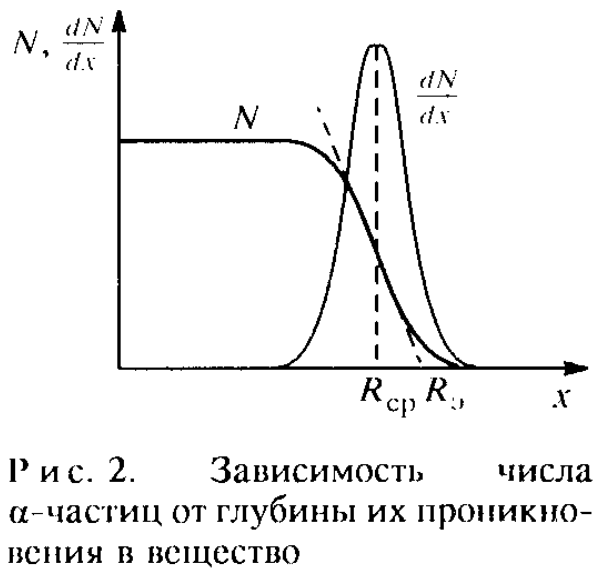
\includegraphics[width = 0.5\linewidth]{A(L)}
\end{figure}

При малых глубинах число частиц не меняется с расстоянием. В конце пути это число не сразу обрывается до нуля, а приближается к нему постепенно. Как видно из кривой $\frac{dN}{dx}$, большая часть $\alpha$-частиц останавливается в узкой области, расположенной около некоторого значения $x$, которое называется средним пробегом $R_{ср}$. В формулу (12) входит именно $R_{ср}$. Иногда вместо $R_{ср}$ измеряют экстраполированный пробег $R_\textnormal{э}$. Чтобы его получить, нужно продолжить до пересечения с осью $x$ касательную к кривой $N(x)$, взятую в точке $x=R_{ср}$.

Несмотря на наличие коллиматора, в данной работе мы имеем дело не с узкими параллельными пучками частиц, а с пучками конечных размеров, обладающих заметной угловой расходимостью. Это приводит к тому, что экспериментально наблюдаемые зависимости числа $\alpha$-частиц от глубины их проникновения качественно правильно передают появление брэгговского пика и, тем самым, относительную величину пробега частиц с разной энергией. Однако в силу указанных причин брэгговский пик оказывается смещенным и сильно размытым. Поэтому лучшей оценкой пробега оказывается экстраполированный пробег.

При экспериментальном исследовании пробега $\alpha$-частиц следует помнить, что источники $\alpha$-частиц могут загрязнять близлежащие поверхности. Это происходит из-за отдачи, которую испытывают атомы при испускании $\alpha$-частиц. Чтобы избежать такого загрязнения, источники $\alpha$-частиц обычно покрывают пленкой. Какой бы тонкой ни была защитная пленка, она вызывает некоторое замедление $\alpha$-частиц.

В качестве источника $\alpha$-частиц используется $^{239}Pu$ с периодом полураспада $T_{\frac{1}{2}}=2,44\cdot10^4$  лет. Альфа-частицы, испускаемые $^{239}Pu$, состоят из трех моноэнергетических групп, различие между которыми лежит в пределах 50 кэВ. При той точности, которая достигается в наших опытах, их можно считать совпадающими по энергии, равной $\sim 5$ МэВ. 
% section теоритическая_часть (end)
\newpage
\section{Определение пробега $\alpha$-частиц с помощью сцинтилляционного счетчика} % (fold)
\label{sec:определение_пробега_alpha_частиц_с_помощью_сцинтилляционного_счетчика}

\begin{table}[h!]
	\centering
	\caption{Измерение числа зарегестрированных частиц за определенный период, при измеренном давлении}
	\begin{tabular}{|c|c|} 
			\hline	
			Период, c&  число частиц\\
			\hline
			\multicolumn{2}{|c|}{При давлении 20 мм. рт. ст.}\\ \hline
			10	&	3716	\\ \hline
			10	&	3762	\\ \hline
			10	&	3613	\\ \hline
			10	&	3549	\\ \hline
			10	&	3543	\\ \hline
			10	&	3627	\\ \hline
			100	&	36431	\\ \hline
			100	&	37167	\\ \hline
			\multicolumn{2}{|c|}{При давлении 60 мм. рт. ст.}\\ \hline
			10	&	3428	\\ \hline
			10	&	3373	\\ \hline
			10	&	3475	\\ \hline
			10	&	3403	\\ \hline
			10	&	3531	\\ \hline
			10	&	3416	\\ \hline
			\multicolumn{2}{|c|}{При давлении 80 мм. рт. ст.}\\ \hline
			10	&	3322	\\ \hline
			10	&	3235	\\ \hline
			10	&	3245	\\ \hline
			10	&	3164	\\ \hline
			10	&	3171	\\ \hline
			10	&	3217	\\ \hline
			10	&	3408	\\ \hline
			10	&	3262	\\ \hline
			10	&	3398	\\ \hline
			\multicolumn{2}{|c|}{При давлении 110 мм. рт. ст.}\\ \hline
			10	&	2978	\\ \hline
			10	&	3049	\\ \hline
			10	&	2914	\\ \hline
			10	&	2997	\\ \hline
			
			
	\end{tabular}
	\begin{tabular}{|c|c|}
		\hline	


		\multicolumn{2}{|c|}{При давлении 110 мм. рт. ст.}\\ \hline
		10	&	2918	\\ \hline
		10	&	2885	\\ \hline
		10	&	2863	\\ \hline
		10	&	2922	\\ \hline
		\multicolumn{2}{|c|}{При давлении 130 мм. рт. ст.}\\ \hline
		10	&	2858	\\ \hline
		10	&	2798	\\ \hline
		10	&	2786	\\ \hline
		10	&	2720	\\ \hline
		10	&	2742	\\ \hline
		10	&	2720	\\ \hline
		10	&	2768	\\ \hline
		10	&	2743	\\ \hline
		\multicolumn{2}{|c|}{При давлении 150 мм. рт. ст.}\\ \hline
		10	&	2493	\\ \hline
		10	&	2473	\\ \hline
		10	&	2562	\\ \hline
		10	&	2504	\\ \hline
		10	&	2478	\\ \hline
		10	&	2454	\\ \hline
		10	&	2511	\\ \hline
		10	&	2481	\\ \hline
		\multicolumn{2}{|c|}{При давлении 180 мм. рт. ст.}\\ \hline
		10	&	1939	\\ \hline
		10	&	1985	\\ \hline
		10	&	1995	\\ \hline
		10	&	2053	\\ \hline
		10	&	1993	\\ \hline
		10	&	1927	\\ \hline
		10	&	1946	\\ \hline
		10	&	1883	\\ \hline
		
		\end{tabular}
	\end{table}

	\begin{table}[h!]
			\centering
		\begin{tabular}{|c|c|}
		\hline		
					\multicolumn{2}{|c|}{При давлении 210 мм. рт. ст.}\\ \hline
					10	&	1350	\\ \hline
					10	&	1429	\\ \hline
					10	&	1384	\\ \hline
					10	&	1357	\\ \hline
					10	&	1333	\\ \hline
					10	&	1417	\\ \hline
					10	&	1367	\\ \hline
					10	&	1386	\\ \hline
					\multicolumn{2}{|c|}{При давлении 240 мм. рт. ст.}\\ \hline
					10	&	858	\\ \hline
					10	&	823	\\ \hline
					10	&	815	\\ \hline
					10	&	801	\\ \hline
					10	&	878	\\ \hline
					10	&	806	\\ \hline
					10	&	873	\\ \hline
					10	&	823	\\ \hline
					\multicolumn{2}{|c|}{При давлении 280 мм. рт. ст.}\\ \hline
					10	&	286	\\ \hline
					10	&	291	\\ \hline
					10	&	265	\\ \hline
					10	&	277	\\ \hline
					10	&	294	\\ \hline
					10	&	286	\\ \hline
					10	&	299	\\ \hline
					10	&	289	\\ \hline
					\multicolumn{2}{|c|}{При давлении 310 мм. рт. ст.}\\ \hline
					10	&	13	\\ \hline
					10	&	9	\\ \hline
					10	&	10	\\ \hline
					10	&	15	\\ \hline
					
			
		\end{tabular}
		\begin{tabular}{|c|c|}
			\hline
			\multicolumn{2}{|c|}{При давлении 310 мм. рт. ст.}\\ \hline
			10	&	14	\\ \hline
			10	&	10	\\ \hline
			10	&	4	\\ \hline
			10	&	11	\\ \hline

			\multicolumn{2}{|c|}{При давлении 340 мм. рт. ст.}\\ \hline
			10	&	2	\\ \hline
			10	&	1	\\ \hline
			10	&	2	\\ \hline
			10	&	4	\\ \hline
			10	&	1	\\ \hline
			10	&	2	\\ \hline
			10	&	1	\\ \hline
			30	&	11	\\ \hline	
			\multicolumn{2}{|c|}{При давлении 430 мм. рт. ст.}\\ \hline
			100	&	53	\\ \hline
			100	&	12	\\ \hline
			10	&	2	\\ \hline
			10	&	3	\\ \hline
			\multicolumn{2}{|c|}{При давлении 560 мм. рт. ст.}\\ \hline
			100	&	7	\\ \hline
			100	&	6	\\ \hline
			10	&	1	\\ \hline
			10	&	2	\\ \hline
			\multicolumn{2}{|c|}{При давлении 660 мм. рт. ст.}\\ \hline
			100	&	10	\\ \hline
			100	&	11	\\ \hline
			10	&	1	\\ \hline
			10	&	1	\\ \hline
		
		\end{tabular}
	\end{table}
	\clearpage
	
	Построим график зависимости N = N(P), (число зарегестрированных в секунду частиц от давления)
	\begin{figure}[h!]
		\centering
		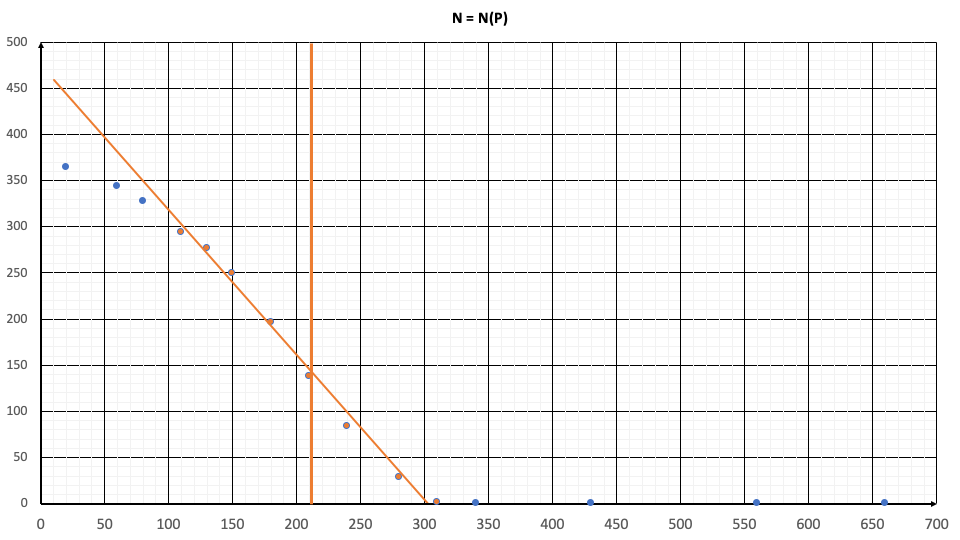
\includegraphics[width =1.1\linewidth]{N(P)}

		\caption{График зависимости $N = N(P)$}
	\end{figure} 
	Уравнение прямой: $y = -1,5712x + 474,66$\\
	По этому уравнению найдем давление $P_0$ при котором пробег 9 см:
	$$
	P_0 = \frac{474,66}{1,57} = 302,1(\textnormal{мм. рт. ст.})
	$$
	Тогда при давлении 760 мм. рт. ст. пробег
	$$
	R = \frac{P}{P_0}\cdot R_0 = 3,6 cm
	$$
	Тогда по формуле $R = 0,32E^{3/2}$ Найдем энергию $\alpha$-частицы:
	$$
	E_{\alpha} = (\frac{R}{0,32})^{2/3}= 5,0 (\textnormal{МэВ})
	$$
	\newpage
% section определение_пробега_alpha_частиц_с_помощью_сцинтилляционного_счетчика (end)
	\section{Определение пробега $\alpha$ - частиц с помощью ионизационной камеры} % (fold)
	\label{sec:определение_пробега_alpha_частиц_с_помощью_ионизационной_камеры}
	\begin{table}[h!]
		\centering
		\caption{Измерение тока при разных давлениях}
		\begin{tabular}{|c|c|}	
			\hline
			I, пА & P, торр. \\ \hline
			76	&	75	\\ \hline
			72	&	70	\\ \hline
			65	&	65	\\ \hline
			57	&	60	\\ \hline
			50	&	55	\\ \hline
			45	&	50	\\ \hline
			37	&	45	\\ \hline
			32	&	40	\\ \hline
			84	&	80	\\ \hline
			92	&	85	\\ \hline
			99	&	90	\\ \hline
			107	&	95	\\ \hline
			114	&	100	\\ \hline
			120	&	105	\\ \hline
			126	&	110	\\ \hline
			
		\end{tabular}
		\begin{tabular}{|c|c|}
			\hline
			I, пА & P, торр. \\ \hline
			134	&	115	\\ \hline
			143	&	120	\\ \hline
			149	&	125	\\ \hline
			157	&	130	\\ \hline
			164	&	135	\\ \hline
			175	&	140	\\ \hline
			179	&	145	\\ \hline
			187	&	150	\\ \hline
			194	&	155	\\ \hline
			201	&	160	\\ \hline
			208	&	165	\\ \hline
			214	&	170	\\ \hline
			223	&	175	\\ \hline
			233	&	180	\\ \hline
			241	&	185	\\ \hline
		\end{tabular}
		\begin{tabular}{|c|c|}
			\hline
			I, пА & P, торр. \\ \hline
			250	&	190	\\ \hline
			257	&	195	\\ \hline
			281	&	210	\\ \hline
			295	&	220	\\ \hline
			313	&	230	\\ \hline
			327	&	240	\\ \hline
			345	&	250	\\ \hline
			363	&	260	\\ \hline
			456	&	315	\\ \hline
			515	&	350	\\ \hline
			536	&	360	\\ \hline
			550	&	370	\\ \hline
			590	&	390	\\ \hline
			630	&	410	\\ \hline
			670	&	430	\\ \hline
			\end{tabular}
			\begin{tabular}{|c|c|}
			\hline
			I, пА & P, торр. \\ \hline
			721	&	460	\\ \hline
			768	&	480	\\ \hline
			822	&	510	\\ \hline
			865	&	530	\\ \hline
			900	&	550	\\ \hline
			917	&	560	\\ \hline
			939	&	580	\\ \hline
			938	&	610	\\ \hline
			945	&	630	\\ \hline
			940	&	660	\\ \hline
			924	&	705	\\ \hline
			922	&	720	\\ \hline
			917	&	730	\\ \hline
			912	&	740	\\ \hline
			906	&	750	\\ \hline
			901	&	760	\\ \hline
		\end{tabular}	
	\end{table}
	
	Построим график зависимости $I= I(P)$
	\begin{figure}[h!]
		\centering
		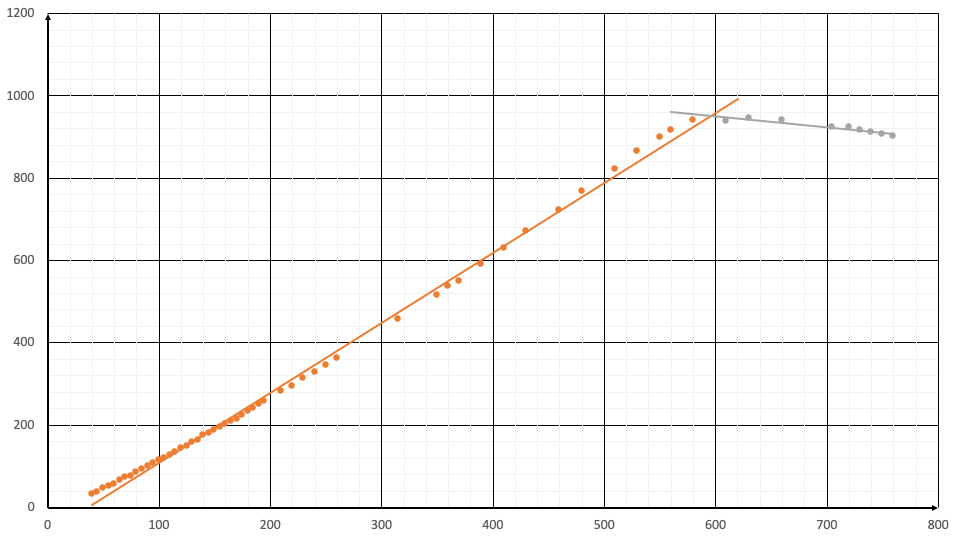
\includegraphics[width = \linewidth]{I(P)}
	\end{figure}
	Уравнения прямых зависимостей I(P) = $-0,3P+1111,8 = 1,7P-62,1$, тогда $$P_0 = \frac{1111,8-62,1}{0,3+1,7} = 532,8\textnormal{Торр}$$
	При этом давлении пробег - 5см, тогда при атмосферном давлении:
	$$R = \frac{532,84\cdot 5}{760} = 3,5 \textnormal{см}$$
	Тогда Энергия $\alpha-$частиц равна
	$$
	E = (\frac{R}{0,32})^{2/3} = 4,9 \textnormal{МэВ}
	$$ 

	% section определение_пробега_alpha_частиц_с_помощью_ионизационной_камеры (end)
	\section{Подсчет погрешностей}
	\label{sec:Подсчет_погрешностей}
	
	 % (fold)
		Для уравнения прямой y = ax+b, по МНК:\\
		\begin{equation}
			a = \frac{<xy> - <x><y>}{<x^2>-<x>^2}	
		\end{equation} 
		\begin{equation}
			b = <y>-a<x>
		\end{equation}
		Погрешность этих коффициентов:
		\begin{equation}
			\sigma_a= \frac{1}{\sqrt{n}} \sqrt{\frac{<y^2>-<y>^2}{<x^2>-<x>^2}-a^2}
		\end{equation}
		\begin{equation}
			\sigma_b=\sigma_a\sqrt{<x^2>-<x>^2}
		\end{equation}
		Сложим независимые погрешности
		\begin{equation}
			\sigma = \sqrt{\sigma_1^2+\sigma_2^2+\sigma_3^2+...}
		\end{equation}
		Для расчета погрешностей воспользуемся формулами (1) - (5)
		 
		Для Энергии в 1 эксперименте:
		$$
			E = 5,0\textnormal{МэВ}
		$$
		$$
			\epsilon = \sqrt{\epsilon_b^2 +\epsilon_a^2} = 5\%\implies
		$$
		$$
			\implies\sigma_E = E \cdot \frac{\epsilon\%}{100\%} = 0,3\implies
		$$
		$$
			\implies E = 5,0\pm 0,3\textnormal{МэВ},\epsilon = 5\%
		$$
		Аналогично для ионизационной камеры:\\
		$$
			\epsilon = 0,1\implies \epsilon\% = 10\%\implies \sigma_E = 0,6\implies E = 4,9\pm0,6\textnormal{МэВ}
		$$
		Тогда графики с ошибками выглядят 
		\begin{figure}[h!]
			\centering
			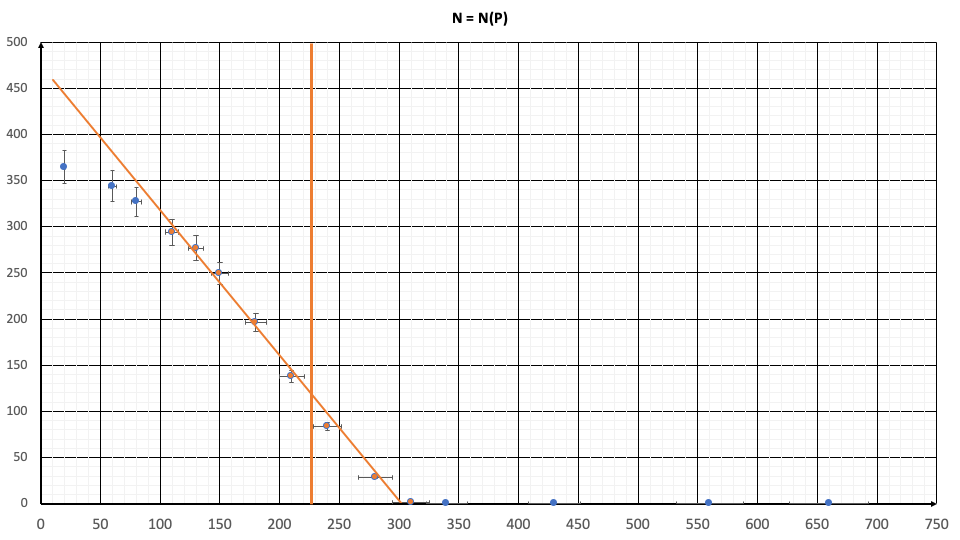
\includegraphics[width = 1.1\linewidth]{N(P)_with_errors}
			\caption{Зависимость N(P) с погрешностями}
		\end{figure}
		\begin{figure}[h!]
			\centering
			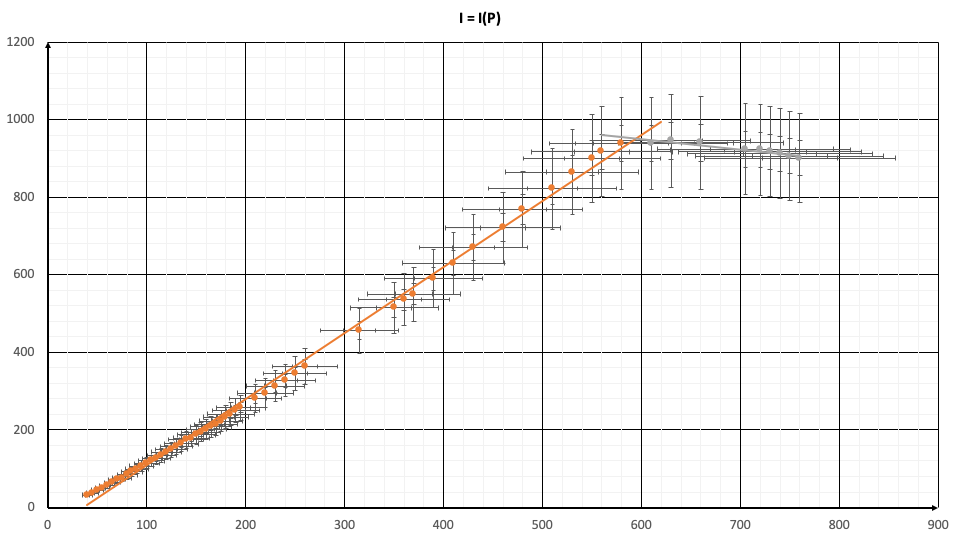
\includegraphics[width = 1.1\linewidth]{I(P)_with_errors}
			\caption{Зависимость I(P) с погрешностями}
		\end{figure}
	% section section_name (end)
	\clearpage
	\section{Итоговый результат:} % (fold)
	\label{sec:Results}
		Измерив пробеги и Энергии $\alpha$ - частиц при нормальных условиях, получили:\\
		\begin{itemize}
			\item Сцинтилляционным счетчиком: $E = 5,0\pm0,3\textnormal{МэВ}$
			\item Ионизационной камерой: $E = 4,9\pm0,6\textnormal{МэВ}$
		\end{itemize}
		Зная, что табличные значения энергии $E = 5,15\textnormal{МэВ}$, то получаем, что оба эксперимента дают верный результат в пределах погрешностей.

	% section Итоговый результат_ (end)

	\section{Вывод} % (fold)
	\label{sec:вывод}
	Я измерил пробег $\alpha$ - частиц в воздухе 2-я способами, и по полученным измерениям определил их энергию.
	% section вывод (end)
\end{document}
